\begin{figure}[htb]
  \centering
%segundo bloco de figuras
  \begin{tabular}{c c c c c }
    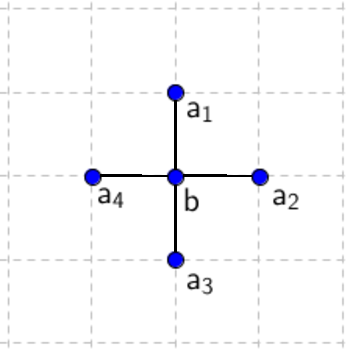
\includegraphics[width=3.5cm]{img/disposicaoTortaGrid3.pdf}    
    & &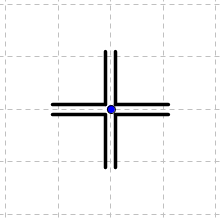
\includegraphics[width=3.5cm]{img/truePieGrid} 
    & &
 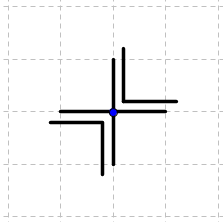
\includegraphics[width=3.5cm]{img/falsePieGrid} \\%[\abovecaptionskip]
    {\footnotesize (a) 4-estrela em uma grade.}  & &  {\footnotesize (b) Torta verdadeira.} & & {\footnotesize (c) Torta falsa.} 
  \end{tabular}
  \caption{Representação $B_{1}$-EPG do ciclo induzido de tamanho  4 como tortas, com ênfase no centro $b$.}\label{fig:piesInGrid}
\end{figure} 